\documentclass[paper.tex]{subfiles}
\begin{document}

\section{Evaluation}
\label{sec:evaluation}

We evaluate \casio on benchmarks drawn from Hamming's \emph{Numerical
  Methods for Scientists and Engineers}~\cite{book87-nmse}, a standard
numerical analysis textbook.  Our evaluation includes
\jdiff{every}{all twenty-eight} worked example\jdiff{}{s} and
problem\jdiff{}{s}\jdiff{, twenty-eight in total,}{} from Chapter~3,
which discusses manually rearranging formulas to improve accuracy, the
same task that \casio automates.

All experiments were carried out on an Intel Core~i5-3317U with 4GB
RAM running Fedora Linux 19, PLT Racket 5.3.6, and GCC 4.9.1.  When
compiling programs to C for performance measurements, we used GCC
flags \texttt{-march=native}, \texttt{-mtune=native},
\texttt{-mfpmath=both}, \texttt{-O3}, and \texttt{-flto}.

Overall, our results demonstrate that \casio can improve accuracy for
many of our benchmarks (\todo{quantitative result here}), often
without significantly slowing execution (\todo{quantitative result
  here}).  In all cases, the programs produced by \casio run orders of
magnitude faster than software floating point (\todo{quantitative
  result here}).  In some cases, the accuracy of the programs output
by \casio even exceeds that solutions provided by experts in numerical
methods textbooks.  We also separately evaluate our error estimation
technique and our regime inference algorithm, and describe several
case studies using \casio.

\begin{figure*}
  \begin{tabular}{cc}
    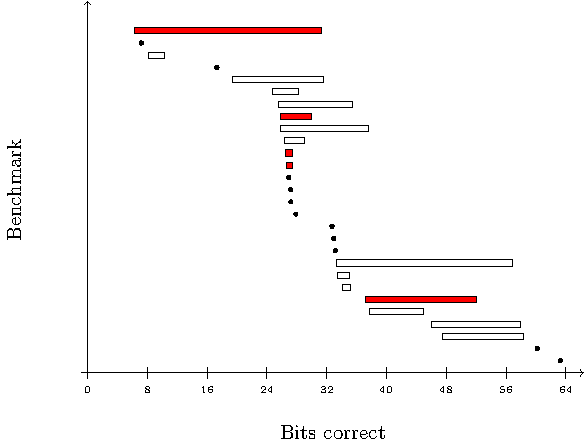
\includegraphics[width=0.9\columnwidth]{fig/eval-rect-f.pdf}
    &
    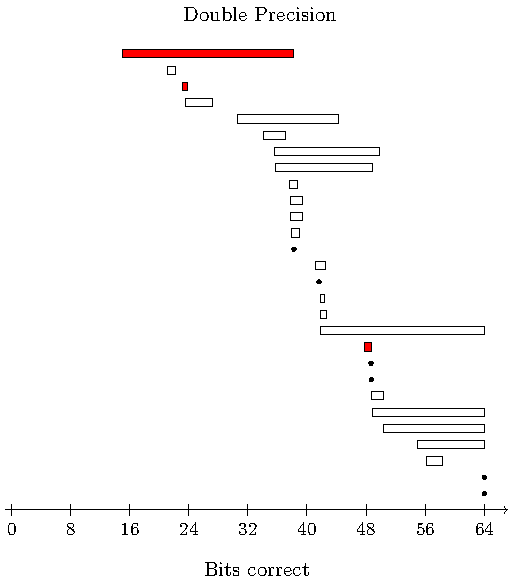
\includegraphics[width=0.9\columnwidth]{fig/eval-rect-d.pdf}
  \end{tabular}
  \caption{Accuracy Results. Each row of the figure represents a
    single benchmark. For each benchmark, the accuracy of the input
    program is drawn as the left edge of a rectangle, and the accuracy
    of \casio's output is drawn as the right edge.  The benchmarks are
    sorted from top to bottom in increasing order of the accuracy of
    \casio's output. The horizontal axis measures accuracy in terms of
    the number of bits of output that agree with the exact result,
    averaged across one million input points. The left half of the
    figure shows results for single precision 32-bit floats, and the
    right half shows results for double precision 64-bit floats. For
    those inputs which \casio is not able to improve by at least half
    a bit, a dot is drawn at the input accuracy level. }
  \label{fig:eval-rect}
\end{figure*}

\para{Accuracy} Our results for both 32-bit single precision floats
and 64-bit double precision floats are shown in
Figure~\ref{fig:eval-rect} .  \jdiff{These results show that \casio
  can successfully improve many of the examples from NMSE.}{}
\todo{more discussion of actual data}. Of the eleven benchmarks that \casio
does not improve, eight have solutions which are not real-equivalent
to the input \jdiff{(Taylor expansions are used to recover precision near 0).
These benchmarks are impossible for \casio to improve without
supporting unsound rewrites.}{because they use Taylor expansions to recover precision
near 0. While \casio cannot currently improve these benchmarks, adding
support for unsound rewrites such as Taylor expansions is an
interesting direction for future work.}

\begin{figure*}
  \begin{tabular}{cc}
    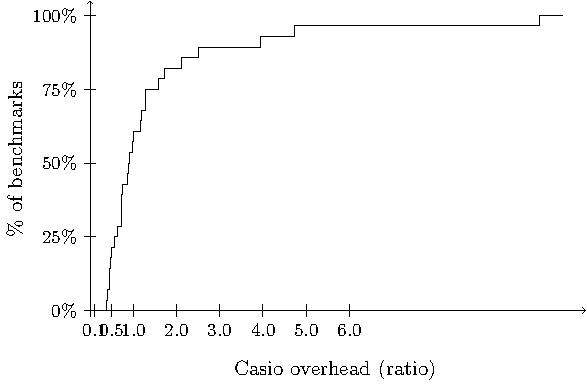
\includegraphics[width=0.9\columnwidth]{fig/eval-overhead-f.pdf}
    &
    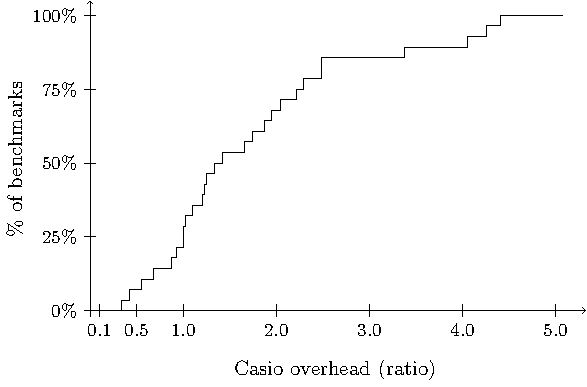
\includegraphics[width=0.9\columnwidth]{fig/eval-overhead-d.pdf}
  \end{tabular}
  \caption{Cumulative distribution of overhead induced by \casio. The
    horizontal axis shows the ratio between the performance of the
    output and input programs. The plot on the left shows results for
    single precision, while the plot on the right shows results for
    double precision. Programs are timed running on one million
    randomly chosen points.}
  \label{fig:eval-overhead}
\end{figure*}

\para{Overhead} We also measured performance overhead.  \jdiff{The timing
measurements demonstrate that \casio does not significantly hurt the
speed of the original program.}{} \casio incurs an average overhead of
\todo{N}\%.  In \todo{N} of the 29 benchmarks, \casio's error with
single precision floating point is greater than the original program's
accuracy with double precision.

\begin{figure}
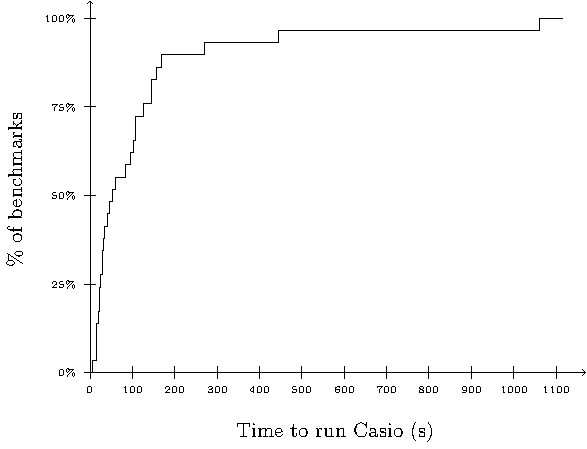
\includegraphics[width=0.9\columnwidth]{fig/eval-casio-time.pdf}
\caption{Cumulative distribution of running time of the \casio tool on
  each benchmark. The horizontal axis shows time in seconds. Most
  benchmarks complete in less than two minutes.}
\label{fig:eval-casio-time}
\end{figure}

\para{Runtime}
\casio was run on each benchmark in a standard configuration%
\footnote{including regime inference and the normal number of sample
  points.}.  The main loop was capped at \nIters iterations.
Figure~\ref{fig:eval-casio-time} is a cumulative distribution function for
\casio's runtime on these benchmarks.  For 17 of 29 tests, \casio runs
in under one minute. \todo{Is the previous sentence accurate?}

\begin{figure}
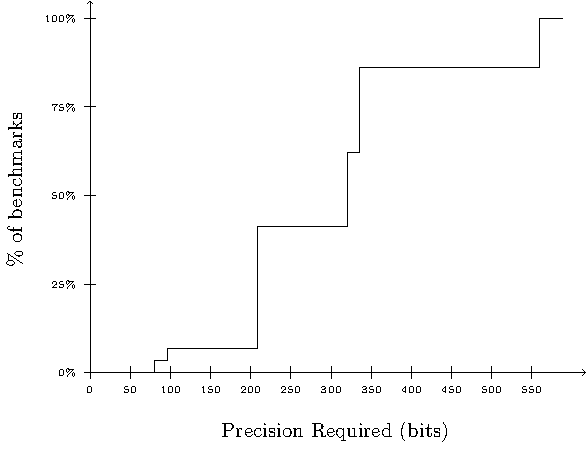
\includegraphics[width=0.9\columnwidth]{fig/eval-mpfr-bits.pdf}
\caption{Cumulative distribution of precision required to evaluate
  each benchmark to 64 bits of accuracy. The horizontal axis shows
  bits of precision. Results were obtained by iteratively increasing
  the precision until the high-order 64 bits converged.}
\label{fig:eval-mpfr-bits}
\end{figure}

\para{Error Estimation}
The accuracy and speed was measured, both for the original program in
each benchmark, and for \casio's output.  Examples were compiled to C,
which was then compiled by the GNU Compiler Collection with flags
optimizing for performance without loss of accuracy%
\footnote{Version $4.9.1$ of \texttt{gcc} was used, with flags
  \texttt{-march=native}, \texttt{-mtune=native},
  \texttt{-mfpmath=both}, \texttt{-O3}, and \texttt{-flto}.
  Experiments were run on an Intel Core~i5-3317U processor.}.
\todo{What about \texttt{-ffast-math}?}  Both the input and output
program were run with single, double, and extended double (32, 64, and
80 bits) intermediates.  Each program was run on the same set of
1,000,000 points drawn randomly from the set of single-precision
floating point numbers.  Results were compared with a ground truth
computed via the MPFR arbitrary-precision library~\cite{acm07-mpfr}.
Figure~\ref{fig:eval-mpfr-bits} shows the cumulative distribution of
the number of bits necessary to exactly evaluate the benchmarks.  The
error of an output computed in floating-point, was taken to be the
base-2 logarithm of the number of 64-bit floating point values%
\footnote{Inputs are single precision values, while outputs are double
  precision.  Single precision for inputs avoids handicapping
  implementations that use single precision for intermediate values.
  Double precision for outputs allows measuring error more accurately
  than single precision would.}, between the exact and inexact answer:
the bits in error for the approximate output, compared to the exact
answer.  This error was averaged over all points for which the exact
answer was a finite floating point value, resulting in a simple number
which can be used for comparing implementations.  Sampling one million
points is a very accurate measure of the average error, as
demonstrated in Section~\ref{sec:eval-eval}.

Average error is a coarse measure of floating point accuracy.  \casio
presents programmers with a graph of error versus input value.  These
plots display 8000 points.  Figure~\ref{fig:err-distr} shows these
plots for \todo{1d program} and \todo{2d program}.  These examples are
representative of all benchmarks.  In all cases, average error
improved when inputs that would produce wholly incorrect results were
changed to producing relatively accurate results.

\subsection{Error Evaluation}
\label{sec:eval-eval}

\begin{figure}
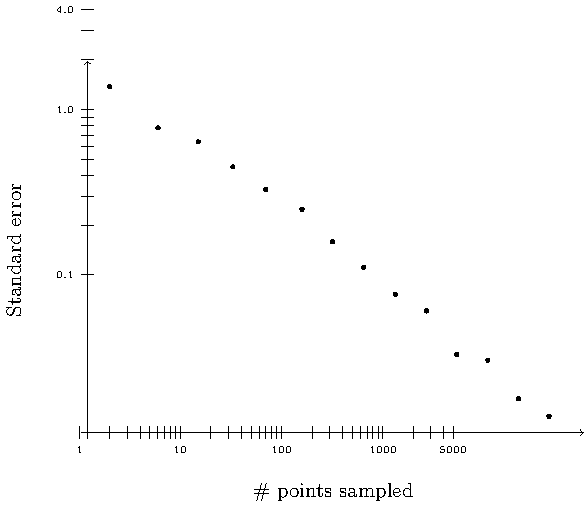
\includegraphics[width=0.9\columnwidth]{fig/eval-err.pdf}
\caption{Standard error vs. sample size. Each point represents one
  hundred runs of \casio on the quadratic formula benchmark with
  varying sample size used to estimate error of program variants. The
  horizontal axis shows the sample size. The vertical axis shows
  standard error of the mean of the error estimates produced by the
  one hundred runs. By default, \casio runs the search with a sample
  size of 500, which has a standard error of approximately 0.1.}

\label{fig:eval-err}
\end{figure}

The tests above evaluated \casio by comparing the average error of its
input and output.  Average error was computed by sampling one million
points and computing the average error across the sample.  To
demonstrate that this accurately estimates average error, we computed
average error with the number of points $N$ varying between 1 and
10,000.  For each $N$, the experiment was repeated 100 times with
different sampled points.  The standard error of the mean of these 100
repetitions, for each value of $N$, measures the accuracy of our
computation of average error.  Figure~\ref{fig:eval-err} is a
representative result; it was generated from the the quadratic formula
example described in Section~\ref{sec:overview}, but every test case
generated a qualitatively similar result.  In each case, sampling a
thousand points gave a result with standard error of approximately
$0.1$ bits.  This demonstrates that the numbers given above are
accurate.

To ensure that our evaluation in arbitrary precision is accurate (that
is, to ensure that we use a sufficiently large number of bits to
evaluate the results accurately), we computed the exact answer for
both \casio's input and output in arbitrary precision.  In every case,
the answers were identical, showing that arbitrary precision
evaluation is accurate. Thus our rewrite are sound.

We have run \casio with sample points being drawn uniformly in the
range $[-\mathsf{max}_{32}, \mathsf{max}_{32}]$, where $\mathsf{max}_{32}$ is the
largest finite value representable in 32 bit floating point.  \casio
was only able to solve five benchmarks from NMSE, of which two were
benchmarks where no improvement is possible and the other three of
which use periodicity analysis and thus use a separate point-sampling
mechanism.  This suggests that the uniformity over floating point
representations, instead of over the range of values, is the correct
measure to use for guiding \casio's search.

\subsection{Regime Inference} \label{sec:eval-regimes}

Two experiments evaluate \casio's regime inference.  The first is an
end-to-end test, running \casio on its standard benchmarks but with
regime inference turned off.  Comparing the results of \casio with and
without regime inference measures the effectiveness of regime
inference.  Regime inference adds branches to eight of the 29
benchmarks; Figure~\ref{fig:eval-regimes-e2e} shows \casio's accuracy
and speed on these eight benchmarks, with and without regime
inference.  The results show that for these test cases, regime
inference significantly improves the accuracy of \casio's results.
However, it also makes the resulting programs slower.  Regime
inference infers branches of the form $a_< < x_i < a_>$, for variables
$x_i$.  Since points are selected randomly, these branches are
impossible for the processor to predict, leading to the large
performance cost.  Practical use may lead to the inferred branch being
predictable; so, the performance cost of regime inference as displayed
in Figure~\ref{fig:eval-regimes-e2e}, is a worst-case cost.

A second experiment measures regime inference in isolation.  An input
point $p$ is chosen and regimes is asked to combine the constant
candidate programs $10$, $20$, $30$, $40$, $50$, and $60$ to most
accurately compute $(\mathsf{if}\:x < p\:\mathsf{then}\:a\:\mathsf{else}\:b)$.
\todo{Actually, we use different functions} Regime inference must
infer a branch of the form $x < p'$, with the correct candidate
programs on each side of this branch; then, the difference between the
computed value $p'$ and the ground truth $p$ measures regime
inference's ability to accurately infer branch conditions.  This
experiment was repeated 100 times.  In each case, regime inference
inferred a branch of the correct form; the difference between $p$ and
$p'$ averages \todo{N}\% (max \todo{N}\%, min \todo{N}\%).  This
suggests that regime inference infers branch conditions very
accurately.

\subsection{Wider applicability}

To test \casio's applicability beyond its standard benchmark suite, we
gathered mathematical formulas from a variety of sources and tested
both their numerical accuracy and \casio's ability to improve it.
These sources included several papers from Volume 89 of Physical
Review; standard definitions of mathematical functions, such as
hyperbolic trigonometric functions, arithmetic on complex numbers; and
approximations to special functions like \textsf{erf} and $\zeta$.  Of the
68 formulas gathered, we found that 20 exhibited significant floating
point inaccuracies.  For these 20 examples, \casio was able to improve
6 with no modifications and without enlarging its database of rules.
This is yet another confirmation that rounding error can arise in the
daily practice of scientists and engineers.  However, it is important
to note that for these examples we have not determined if inaccuracies
arise for valid inputs; and, for formulas \casio was unable to
improve, whether a real-equivalent formula with lower error exists.

\subsection{Case Study: Computing Probabilities}

Many numerical programs are not library functions or textbooks
examples, but are instead simulations or data analysis scripts used by
scientists, engineers, and mathematicians in the course of their work.
The expressions encountered in these programs are more complex and
less structured than examples like~\eqref{eq:ex}.  \casio has
demonstrated success in improving precision in these more-difficult
cases.

A colleague of ours had difficulties with the numerical precision of a
estimator in a machine learning task.  He needed to compute the
expression
\begin{align*}
\mathsf{ans} &= \frac{p(e_-,e_+|s)}{p(e_-,e_+|t)} \\
p(e_-, e_+|x) &= (\operatorname{sig} x)^{e_+} (1 - \operatorname{sig} x)^{e_-} \\
\operatorname{sig}x &= 1 / (1 - e^{-x})
\end{align*}
and found that the simple encoding of this formula as a program lead
to spurious results and violated invariants in later code.  Our
estimates suggest that this simple encoding produces seventeen bits of
error, averaged over floating point values.  To avoid these problems,
our colleague manually manipulated the expression into a form that
seemed not to cause similar problems; our estimates suggest that this
improved variant had ten bits of average error.

Upon hearing of his troubles, we fed the original, simple
implementation to \casio.  \casio produced a program with four bits
average error:
\begin{equation*}
  \operatorname{exp}\left(e_+\ln{\frac{1+e^{-t}}{1+e^{-s}}} +
     e_-\ln{\frac{1-\frac{1}{1+e^{-s}}}
                 {1-\frac{1}{1+e^{-t}}}}\right)
\end{equation*}
\casio obviated the need for manual algebraic manipulation, and
produced superior results with no manual steps.  The low-error program
that \casio produced was of a complexity level such that human
analysts would be unlikely to reproduce the result.  Furthermore, our
attempts to simplify the program into a form more likely to be found
by human analysts have only been able to do so by greatly increasing
its error.  By properly targetting its search, \casio is able to
consider a greater number of viable alternatives than human analysts
are able to, and is capable of producing better results.

\end{document}
